In Figure \ref{fig:three graphs} we show results of the procedure in Section \ref{section:identifying_causal_features} across a range of layers in Pythia-410M.




\begin{figure}
     \centering
     \begin{subfigure}[b]{0.49\textwidth}
         \centering
         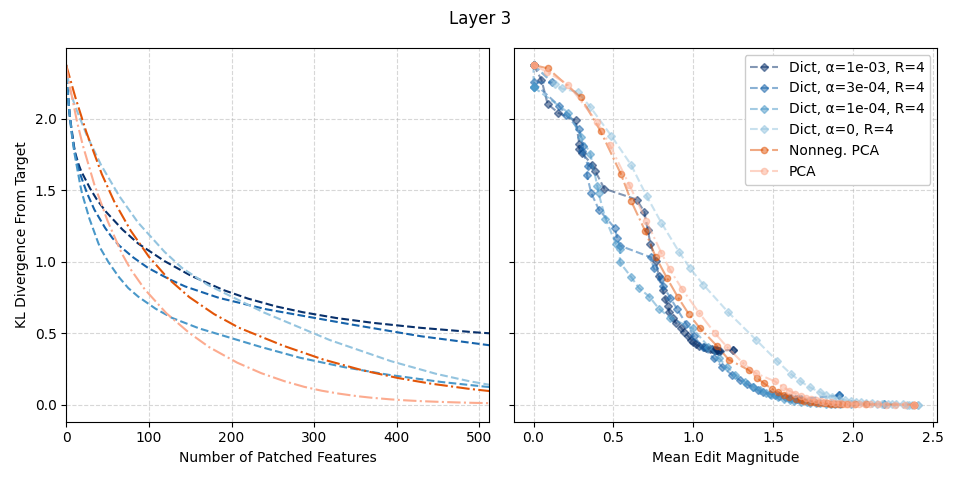
\includegraphics[width=\textwidth]{images/aidan/titled/feature_ident_curve_l3.png}
     \end{subfigure}
     \hfill
     \begin{subfigure}[b]{0.49\textwidth}
         \centering
         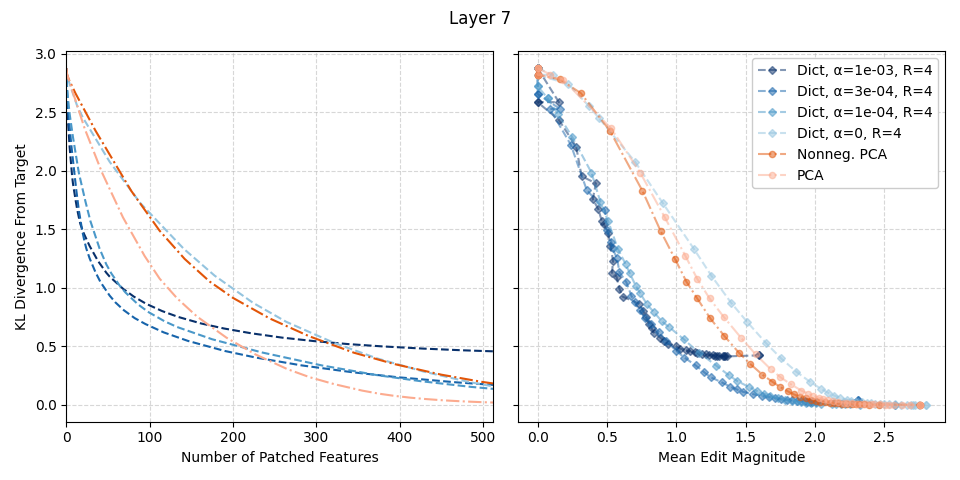
\includegraphics[width=\textwidth]{images/aidan/titled/feature_ident_curve_l7.png}
     \end{subfigure} \\
     \begin{subfigure}[b]{0.49\textwidth}
         \centering
         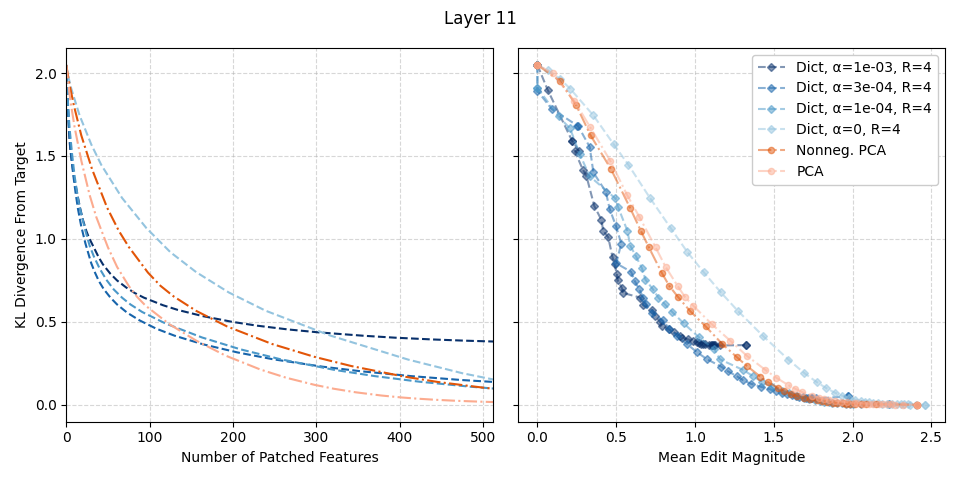
\includegraphics[width=\textwidth]{images/aidan/titled/feature_ident_curve_l11.png}
     \end{subfigure}
     \hfill
     \begin{subfigure}[b]{0.49\textwidth}
         \centering
         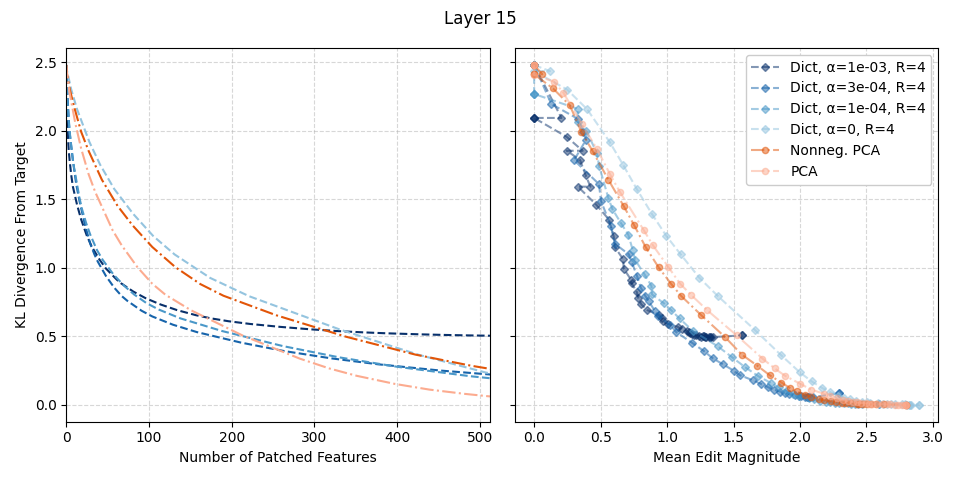
\includegraphics[width=\textwidth]{images/aidan/titled/feature_ident_curve_l15.png}
     \end{subfigure}\\
     \begin{subfigure}[b]{0.49\textwidth}
         \centering
         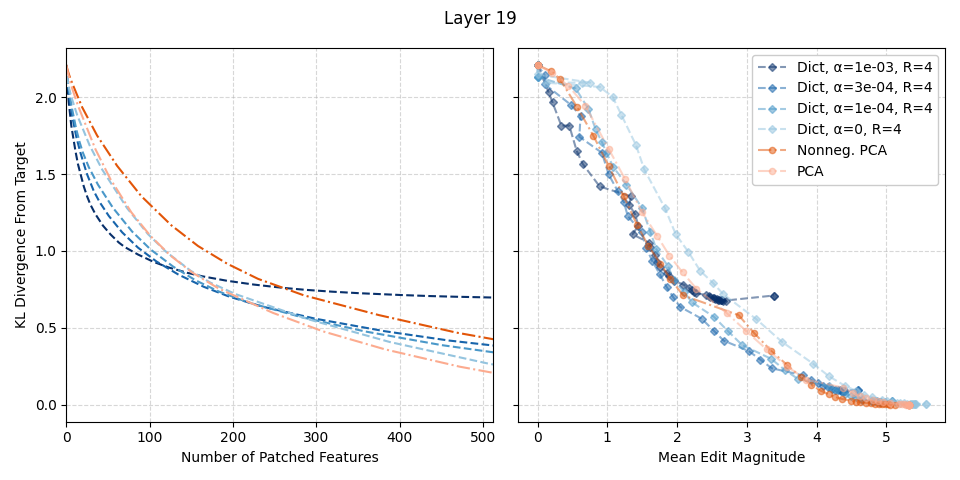
\includegraphics[width=\textwidth]{images/aidan/titled/feature_ident_curve_l19.png}
     \end{subfigure}
     \hfill
     \begin{subfigure}[b]{0.49\textwidth}
         \centering
         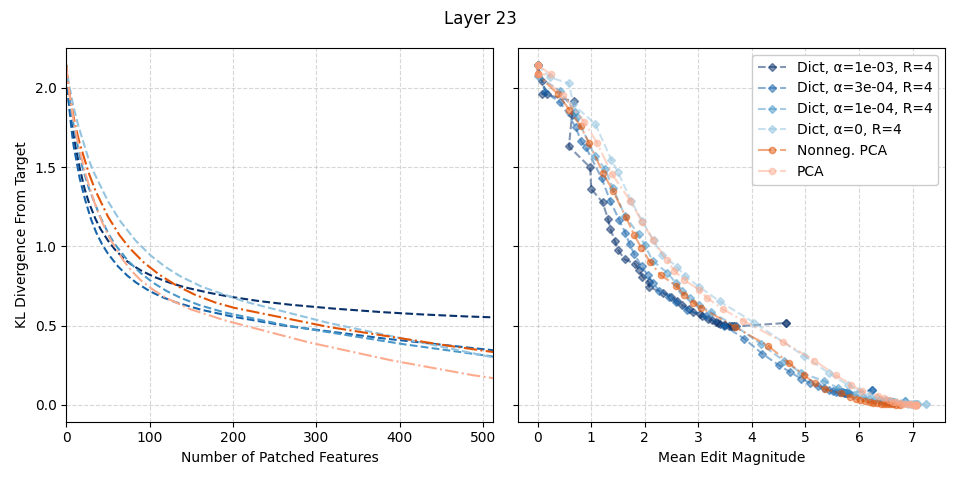
\includegraphics[width=\textwidth]{images/aidan/titled/feature_ident_curve_l23.png}
     \end{subfigure}
        \caption{Divergence from target output against number of features patched and magnitude of edits for layers 3, 7, 11, 15, 19 and 23 of the residual stream of Pythia-410M. Pythia-410M has 24 layers, which we index 0, 1, ..., 23.}
        \label{fig:three graphs}

\end{figure}
